\chapter{Spécifications}

\paragraph{}
Dans ce chapitre nous allons expliquer les fonctionnalités du site de rencontre \textit{Adopte Un Inge}. Certaines d'entre elles ne sont malheureusement pas implémentées par manque de temps car nous avons préféré privilégier la qualité du code pour les fonctionnalités déjà développées.
\section{Fonctionnalités}

\nomFonction{Création d'un compte}
\begin{itemize}
 \item Un compte utilisateur est défini par un numéro d'identification, un nom, un prénom, un age, si il est administrateur, une valorisation, une ville, un département, un nombre de likes, un nombre de signalement, son sexe, son orientation, une photo de profil, un mot de passe, une description et un email. Tous les champs ne sont pas obligatoires. En effet lors de la création une description n'est pas demandée par exemple.
 \item Si tous les champs ne sont pas remplis ou si l'email n'est pas un email valide, des messages d'erreurs doivent être affichés.
\end{itemize}

\nomFonction{Connexion}
\begin{itemize}
 \item L'utilisateur doit entrer son adresse mail et son mot de passe dans un formulaire et valider afin de se connecter.
 \item Le site vérifie le couple email / mot de passe ; en cas d'erreur, l'utilisateur est redirigé vers la page de connexion.
 En cas de succès, il est connecté et redirigé vers la page de recherche du site.
\end{itemize}

\nomFonction{Affichage du profil}
\begin{itemize}
 \item L'utilisateur peut visualiser son profil via un bouton placé sur la barre de navigation situé sur la gauche du site.
 \item Les informations affichées sont celles utiles à l'utilisateur, soit son nom, son prénom, son age, son adresse e-mail, sa ville, son département, son sexe, son orientation et sa description.
\end{itemize}

\nomFonction{Editer un profil}
\begin{itemize}
 \item L'accès à la page d'édition d'un profil s'effectue via un bouton placé sur la page de profil de l'utilisateur (il ne peut modifier un profil autre que le sien).
 \item L'utilisateur modifie ses informations (celles affichées sur son profil et son mot de passe).
 \item Afin d'enregistrer ses modifications il appuie sur un bouton confirmant sa ou ses modifications.
\end{itemize}


\nomFonction{Rechercher}
\begin{itemize}
 \item La recherche s'effectue via la barre de navigation.
 \item La recherche est filtrée à l'aide des critères suivants : âge, ville et département.
 \item La recherche affiche les utilisateurs satisfaisants les critères renseignés.
\end{itemize}

\nomFonction{Afficher un profil autre que le sien}
\begin{itemize}
 \item L'accès à la page de profil d'un utilisateur s'effectue par un clic sur un membre affiché par la recherche.
 \item Affiche la page de profil du membre.
\end{itemize}

\nomFonction{Liker}
\begin{itemize}
 \item Un utilisateur peut "liker" un autre utilisateur.
 \item Le nombre de "like" s'incrémente de un en fonction de si l'utilisateur a "liké" ou non le deuxième utilisateur.
\end{itemize}


\nomFonction{Chat}
\begin{itemize}
\item Pour avoir accès au chat on peut: cliquer sur chat sur la barre de navigation, cliquer sur un bouton contacter sur un profil utilisateur.
\item Si on clique sur la barre de navigation on est redirigé vers une page contenant toutes les conversations.
\item Si on clique sur une conversation on est alors redirigé sur le chat liant les deux utilisateurs entre eux.
\item Nous n'avons malheureusement pas réussi à finir cette fonctionnalité de manière optimale.
\end{itemize}

\nomFonction{Déconnexion}
\begin{itemize}
 \item L'utilisateur peut se déconnecter via un bouton placé sur la barre de navigation logout.
  L'utilisateur est alors redirigé vers la page de connexion et d'inscription (cette fonctionnalité bugue car si on utilise le retour du navigateur nous sommes de nouveau connecté bien que nous avons utilisé la fonction invalidate() de struts2 sans succès).
\end{itemize}

\nomFonction{Fonctionnalités non créées}
Comme dit dans l'introduction du chapitre nous n'avons pas pu implémenter toutes les fonctionnalités que nous voulions en début de projet par manque de temps.
\begin{itemize}
\item La fonctionnalité de valorisation d'un utilisateur n'a ainsi pas pu être faite.
\item La fonctionnalité de création d'évènements n'a ainsi pas pu être faite.
\item La fonctionnalité de signalisation d'un utilisateur n'a ainsi pas pu être faite.
\item La gestion des photos de profils n'a ainsi pas pu être faite
\end{itemize}

\newpage
\section{Diagrammes de cas d'utilisation et diagramme de navigation}

Voici quelques diagrammes de cas d'utilisation et le diagramme de navigation réalisés lors de la conception du projet. Le diagramme de navigation contient des pages qui n'ont pas pu être développé par manque de temps comme dit précédemment.
\vfill
\begin{figure}[ht!]
  \centering
   \caption{Diagramme de cas d'utilisation de création d'un compte}
   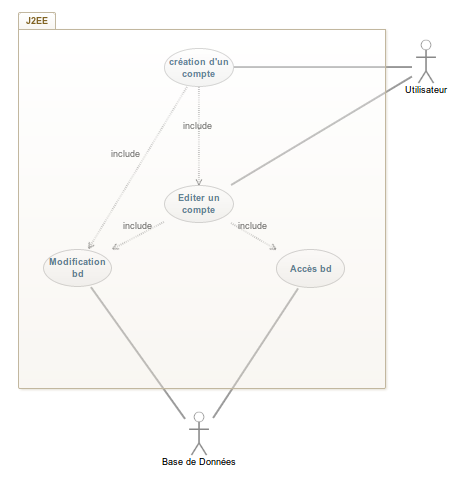
\includegraphics[scale=0.7]{cuCC}
\end{figure}

\begin{figure}[ht!]
  \centering
   \caption{Diagramme de cas d'utilisation du chat}
   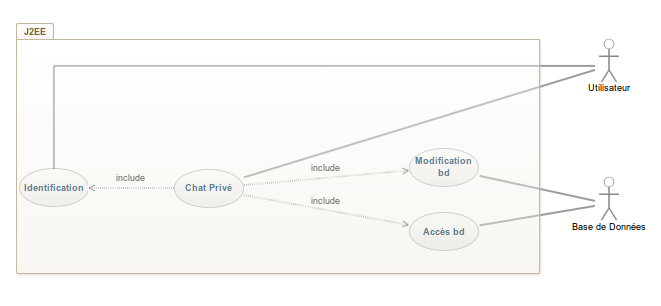
\includegraphics[scale=0.6]{cucp}
\end{figure}

\begin{figure}[ht!]
  \centering
   \caption{Diagramme de cas d'utilisation d'affichage d'un profil}
   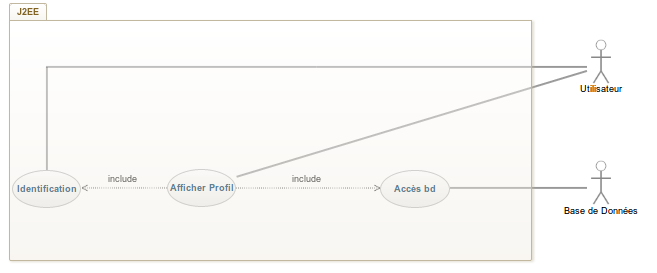
\includegraphics[scale=0.6]{cuAP}
\end{figure}

\begin{figure}[ht!]
  \centering
   \caption{Diagramme de cas d'utilisation d'édition d'un profil}
   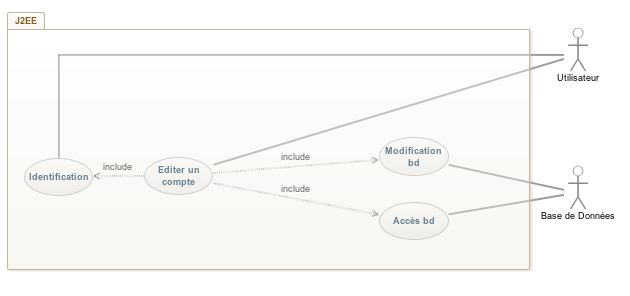
\includegraphics[scale=0.6]{cuEP}
\end{figure}

\begin{figure}[ht!]
  \centering
   \caption{Diagramme de cas d'utilisation de recherche d'un profil}
   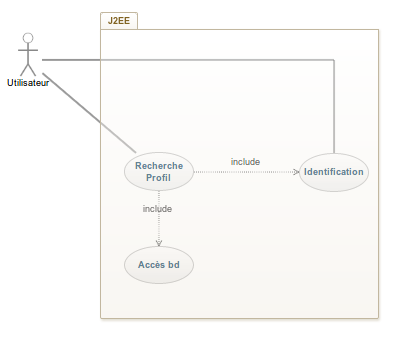
\includegraphics[scale=0.6]{cuRP}
\end{figure}

\begin{figure}[ht!]
  \centering
   \caption{Diagramme de cas d'utilisation d'identification}
   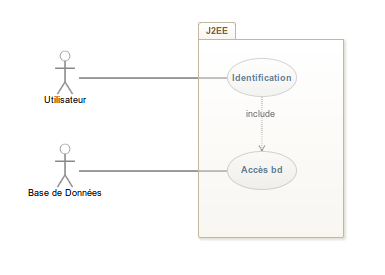
\includegraphics[scale=0.6]{cuId}
\end{figure}

\newpage

  \begin{figure}[ht!]
    \centering
    \caption{Diagramme de navigation}
    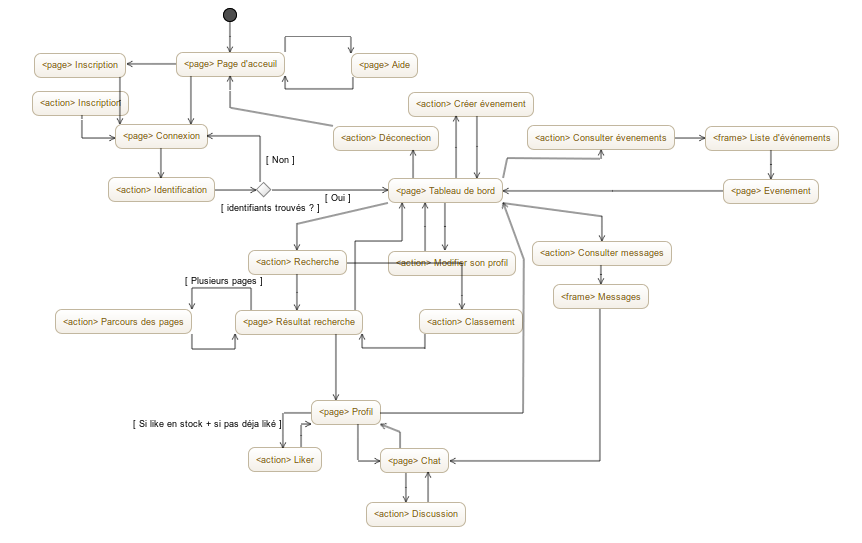
\includegraphics[scale=0.4]{dNav}
  \end{figure}
